\documentclass{article}
\usepackage[english,polish]{babel}
\selectlanguage{polish}

\title{\huge  \Huge \textbf{MOZA Projekt} \\ \textbf{Wzmacniacz Kaskodowy 4 (wariant B)}}
\date{\today}
\author{ \LARGE Jakub Półtorak}

\usepackage{amsmath}
\usepackage{amsfonts}
\usepackage{graphicx}
\usepackage[T1]{fontenc}
\usepackage{pdflscape}
\usepackage{rotating}

\begin{document}
\maketitle
\pagenumbering{gobble}
\newpage
\pagenumbering{arabic}
\tableofcontents

\pagebreak

\begin{center}
	\title{ \huge \textbf{Etap 1}}
\end{center}


\section*{Opis problemu}
Zadanie polega na doborze wartości elementów wzmacniacza tak, aby uzyskać makymalnie duży iloczyn
GBW. Na układ nałożono dodatkowe ograniczenia w postaci minimalnego wzmocnienia dla małych częstotliwości $k_{u0} > 10 dB$ oraz minimalnej częstotliwości
granicznej $f_g > 200 MHz$ (rozumianej jako częstoliwość spadku o 3 dB względem $k_{u0}$).
\section{Sformułowanie matematyczne zadań optymalizacji}
Poszukiwane jest minimum funkcji celu:
\[ \min\limits_{\textbf{x}\in \mathbf{R}^+  } f(\textbf{x}) \]
p.o.
\[ g_{i}(\textbf{x}) \leq 0 \ \ \ \  i=1..n_g\]
gdzie:
\[ f(\textbf{x}) = -(k_{u0}\cdot f_g)\]
\(\textbf{x}\) - wektor zmiennych optymalizowanych: \\
\begin{center}
	$\textbf{x}$ =
	$\begin{bmatrix}
			REE1 & REE2 & RE & RC2 & RC3 & CEE & CG
		\end{bmatrix}$,
\end{center}
\(k_{u0}\) - wzmocnienie dla małych częstoliwości, rozumiane jako wzmocnienia dla częstoltiwości 1 kHz.\\
\(f_{g}\) - częstoliwość graniczna, rozumiana jako częstotliwość, dla której wzmocnienie
spada o 3 dB względem $k_{u_{0}}(\textbf{x}) $.

Parametry $k_{u0}(\textbf{x})$ oraz $f_g(\textbf{x})$ obliczane są w Matlabie na pdostawie surowych danych ($U^{AC}_{out}(x,f)$) zwaracnych
przez symulator LTSpice.

Dodatkowo, w zadaniu pojawiają się ogarniczenia nieliniowe związane z wymaganiami projektowymi:\\
\begin{itemize}
	\item \(g_1(\textbf{x}): -(\frac{k_{u0}(\textbf{x})}{k_{u_{min}}}-1) <  0\) \\ Warunek minimalnego wzmocnienia, $k_{umin}=20dB$
	\item \(g_2(\textbf{x}): -(\frac{{f_g}(\textbf{x})}{f_{g_{min}}}-1)<0\) \\ Warunek minimalnej częstotliwości granicznej, $f_{gmin}=200 MHz$
	\item \(g_3(\textbf{x}): b(\textbf{x})-b_{max}<0\) \\ Ograniczenie podbicia charakterystyki, $b_{max}=1dB$. Podbicie $b$ rozumiane jest jako różnica między maksymalnym poziomem wzmocnienia a $k_{u0}$.Podbicie jest obliczane w Matlabie.

\end{itemize}



\section{Wyznaczenie przybliżenia początkowego rozwiązania}
Zgodnie z poleceniem zmodyfiokowano domyślne parametry tak, aby uzyskać rozwiąznie spełniające warunek minmalnej częstotliwości granicznej i wzmocnienia.
Ostatecznie, po wybraniu wartości, wektor \textbf{x} wygląda następująco:
\begin{center}
	$\textbf{x}$ =
	$\begin{bmatrix}
			5\Omega & 15\Omega & 320\Omega & 220\Omega & 200\Omega & 45p & 50p
		\end{bmatrix}$,
\end{center}

Wyniki w punkcie początkowym można zobaczyć na poniższym wykresie:

\begin{figure}[h]
	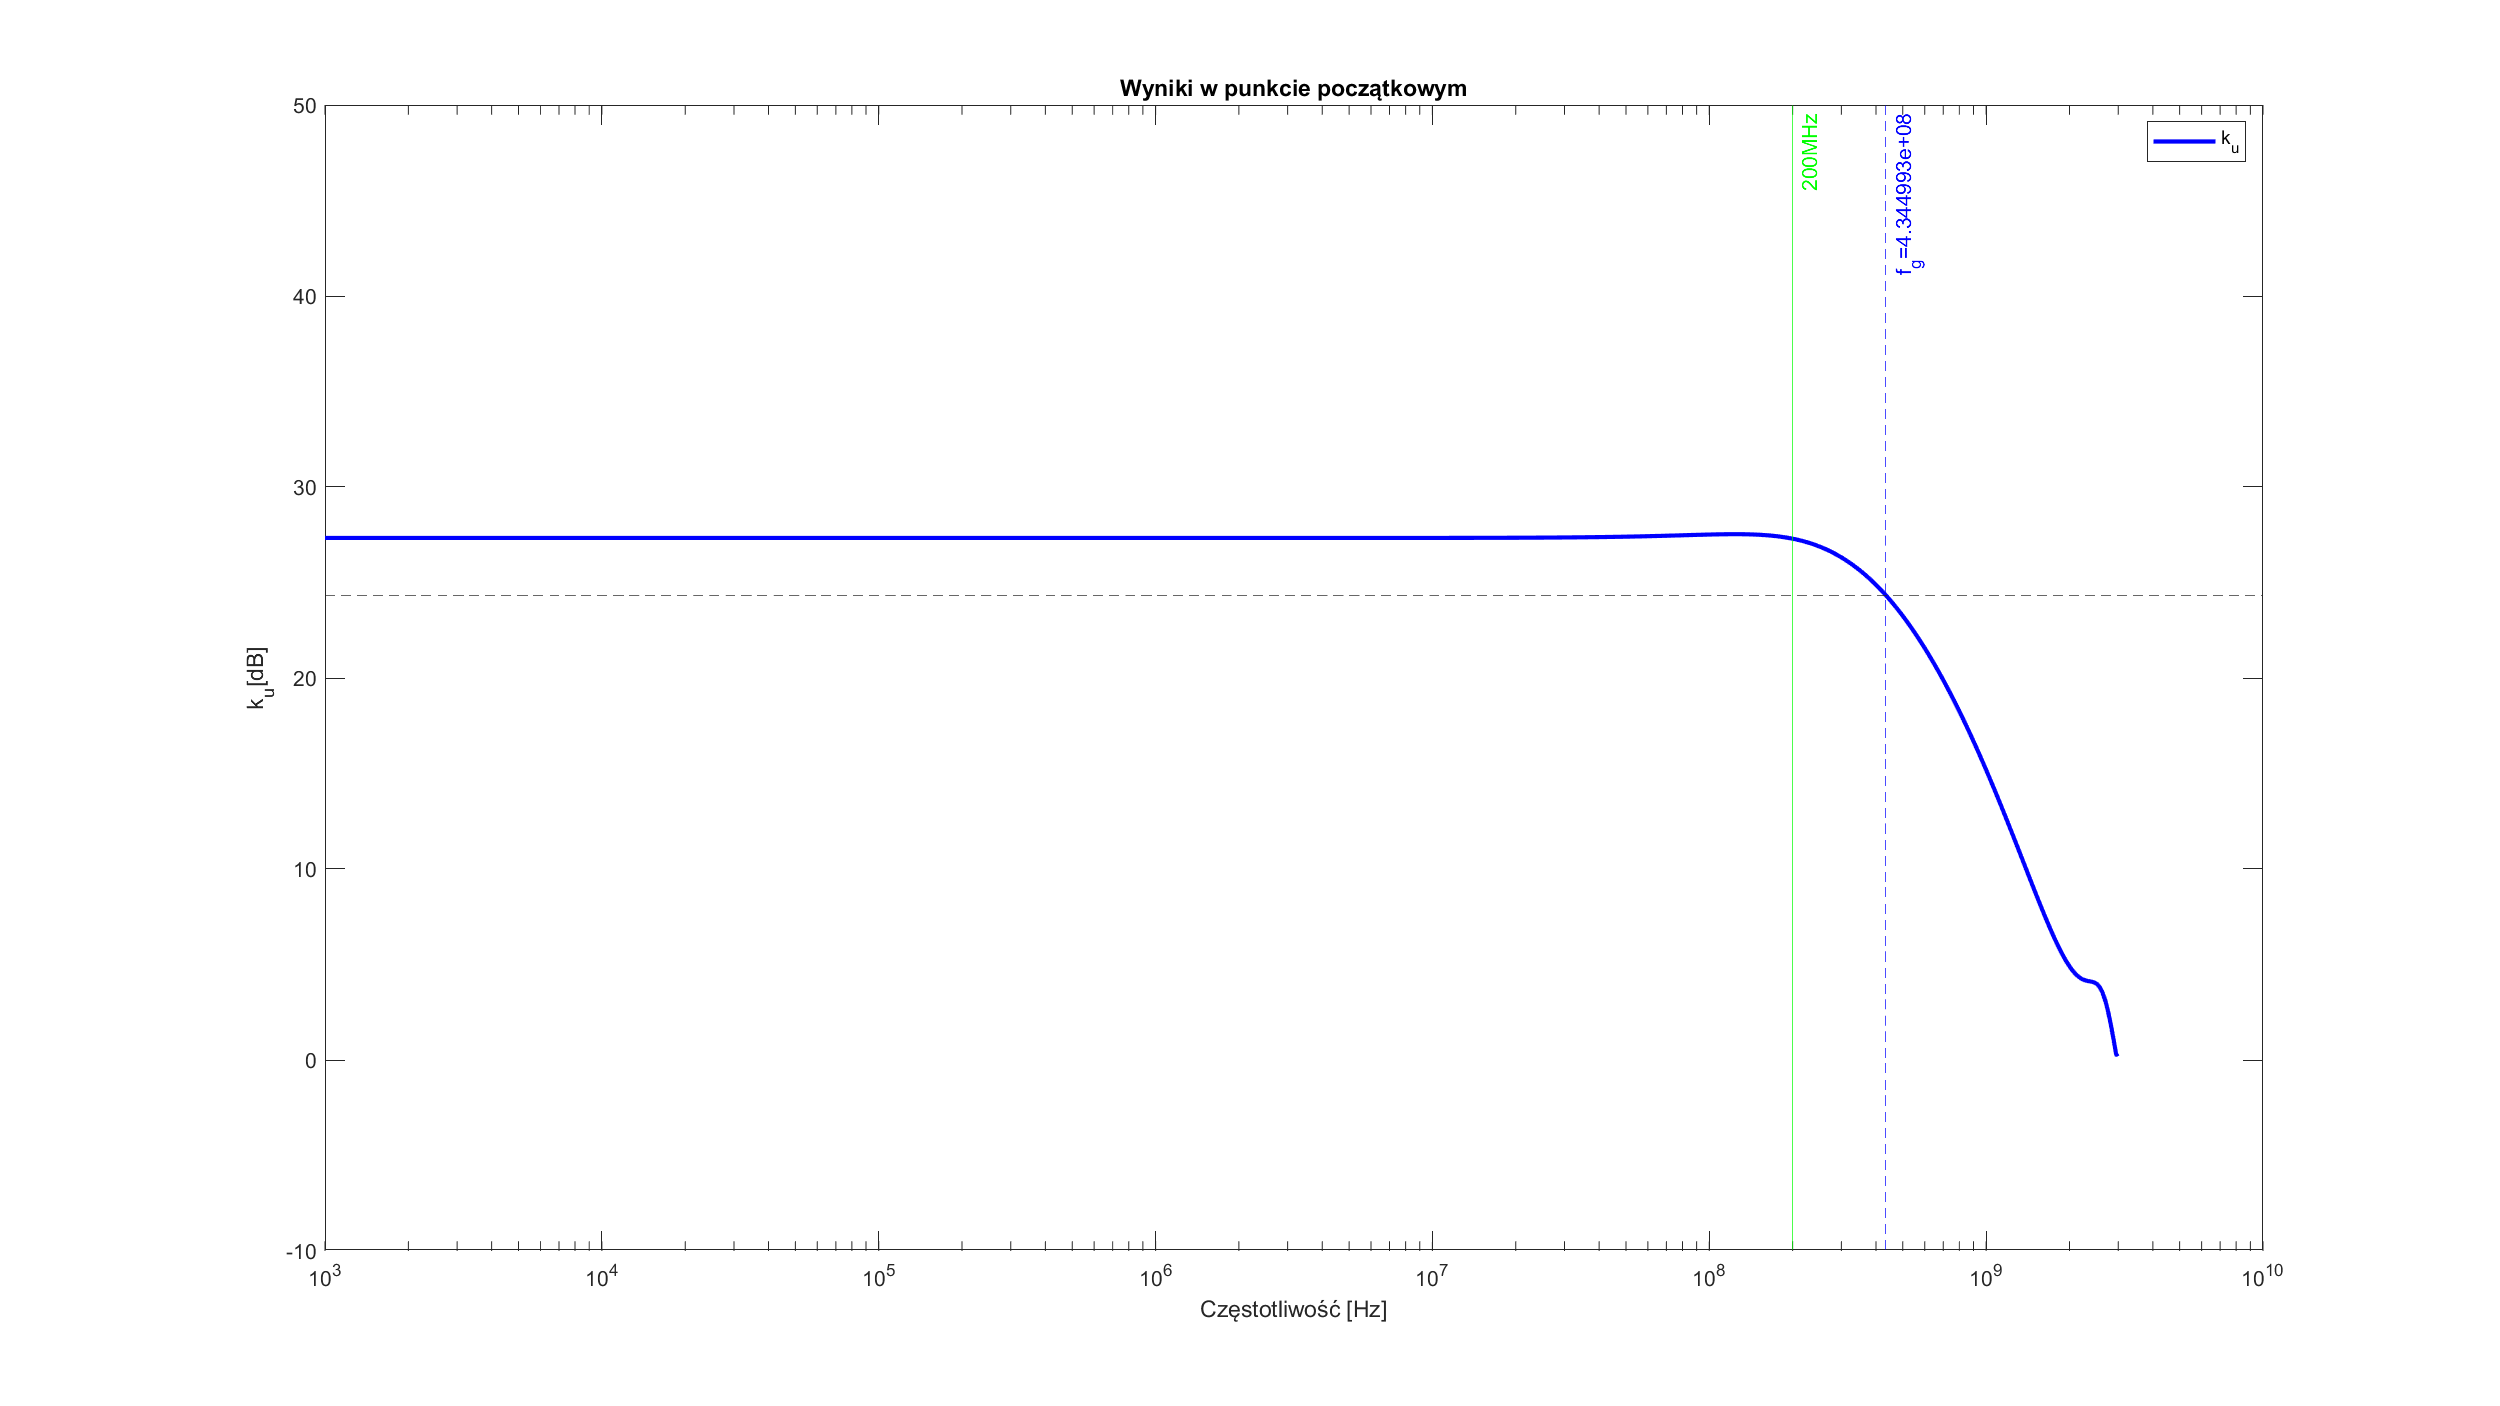
\includegraphics[width=12cm]{graphics/starting_point.png}
	\centering
	\caption{Charakterystyka układu w punkcie startowym.}
\end{figure}

Jak widać spełnione są warunki postawione w zadaniu (minimalna wartość wzmocnenia to 20 dB, przy źródle AC mającym 1V amplitudy) oraz wzmacniacz pracuje prawidłowo.
\pagebreak

Aby potwierdzić, że Matlab i Spice zwracją te same wyniki przeprowadzono symulację w LTSpice:
\begin{figure}[h]
	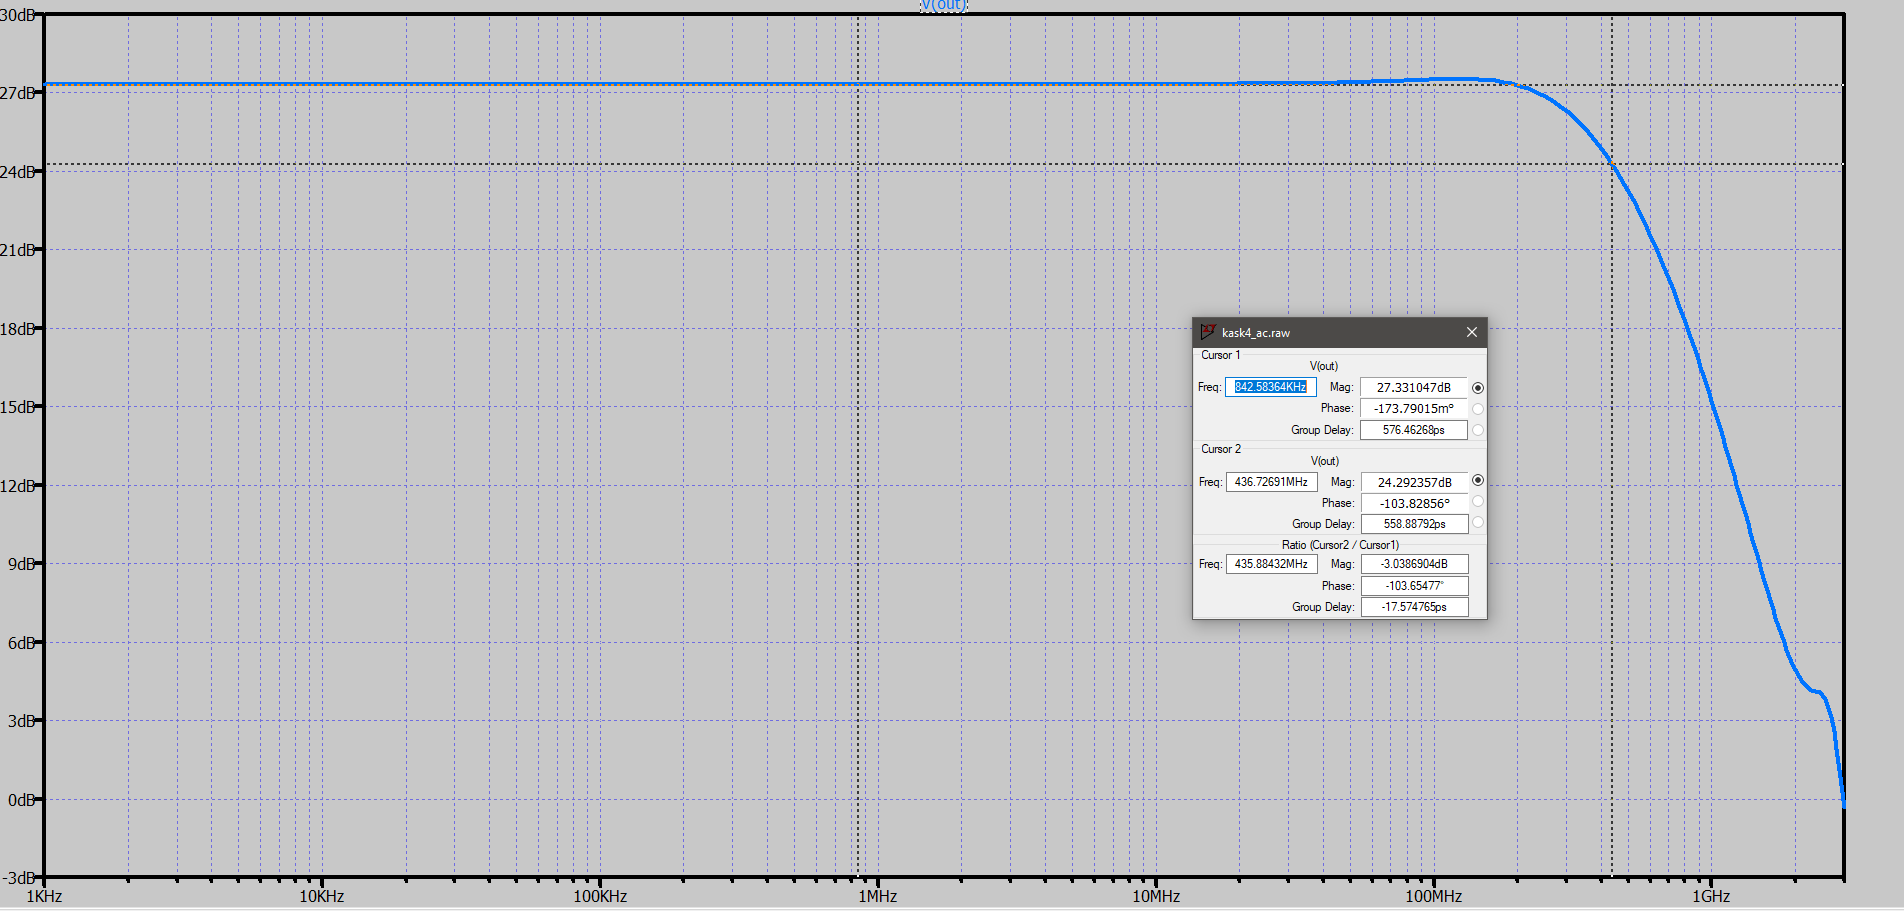
\includegraphics[width=12cm]{graphics/starting_point_spice.png}
	\centering
	\caption{Charakterystyka układu w punkcie startowym.}
\end{figure}


\section{Wyznaczanie parametrów roboczych, gładkość funkcji celu, opis kodu}
\subsection{Wyznaczanie parametrów roboczych}
W zadaniu badane są trzy parametry: częstotliwość graniczna, wzmocnienie oraz podbicie charakterystyki.

\subsubsection*{Podbicie $b$}
Podbicie rozumiane jest jako różnica między wzmocnieniem $k_u0$ a maksymalnym wzmocnieniem jakie osiąga charakterystyka.
\subsubsection*{Wzmocnienie małoczęstotliwościowe $k_u0$}
Wzmocnienie $k_u$ rozumiane jest jako wartość wzmocnienia pozyskana z danych $U^{AC}_{out}(x,f)$ dla częstotliwości 1 KHz.

\subsubsection*{Częstotliwość graniczna $f_g$}
Częstotliwość graniczna wyznaczana jest jako częstotliwość, dla której wzmocnienie względem $k_{u{_0}}$ spada o 3 dB.
Ponieważ LTSpice zwraca wyniki w postaci punktów, uznano, że wymagana jest interpolacja częstotliwości granicznej. Interpolacja pozwoliła zminimalizaować "skoki" w funkcji celu. Do interpoalcji wykorzystano wielomian drugiego stopnia. Wynik interpolacji przedstawia poniższy wykres:
\begin{figure}[h]
	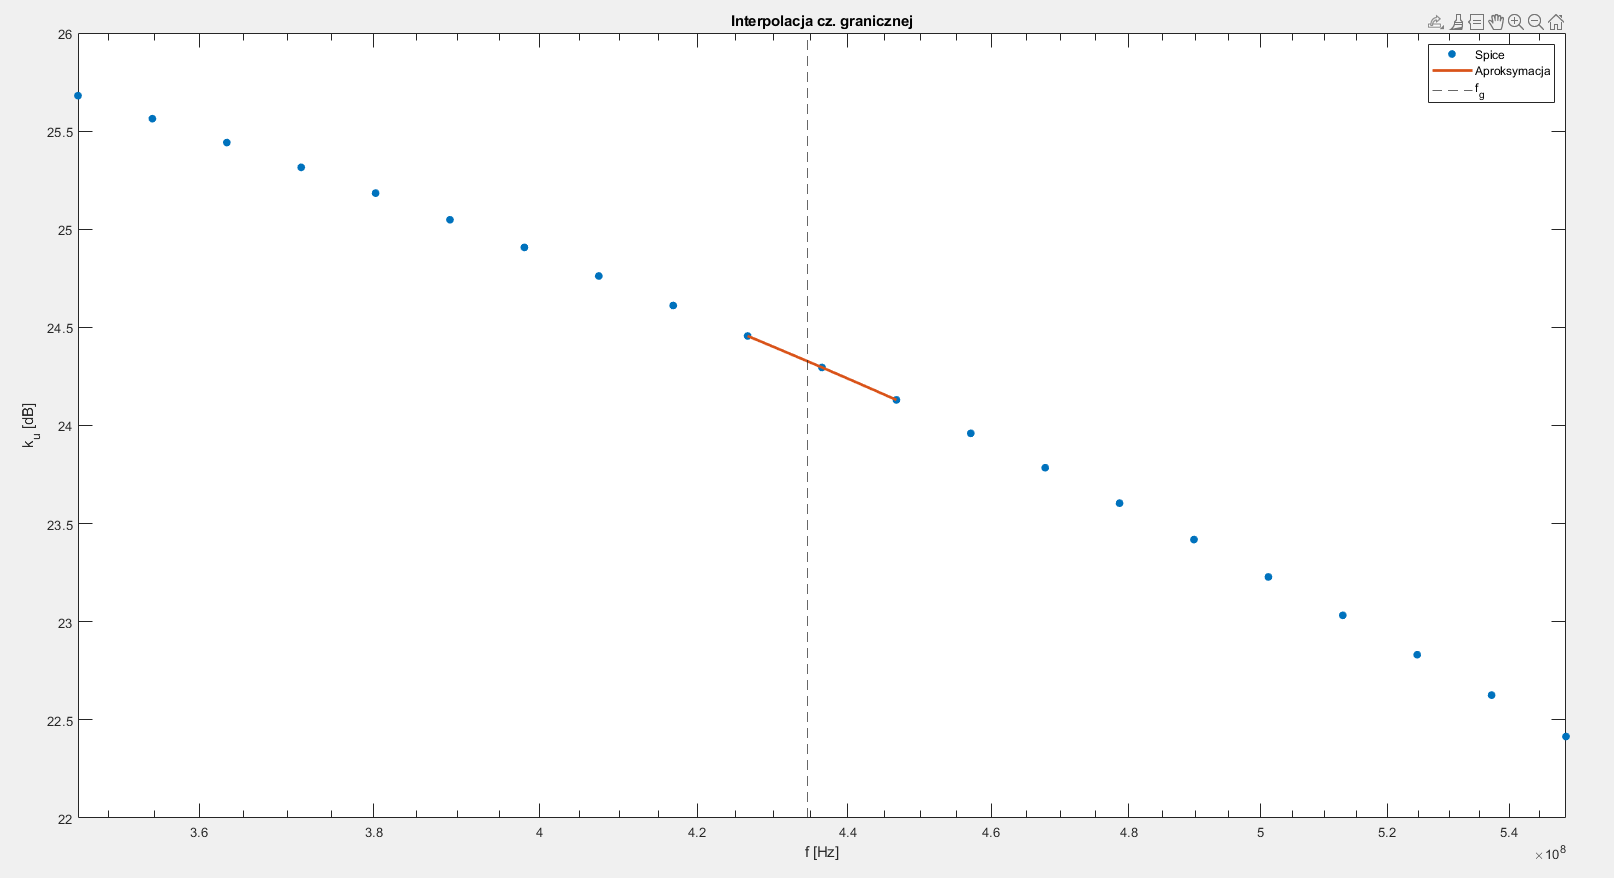
\includegraphics[width=8cm]{graphics/fg_interp.png}
	\centering
	\caption{Interpolacja częstotliwości granicznej.}
\end{figure}




\subsection{Gładkość funkcji celu}
Przyjęto, że funkcja celu, w borębie odpowiednich wartości elemntów układu, jest ciągła. Tak długo, w układzie zmieniane są wartości pojemności i rezystancji i
nie powodują nieprawidłowej pracy układu zawsze możliwe będzie otrzymanie charaktertystyki, która, nawet jeśli nie spełnia wymagań projektowych, otrzymanie prawidłowej odpowiedzi (bez dużych skoków
np. wzrost wzmocnienia do 10000 dB).
\subsection{Opis kodu}
Dołączony katalog z kodem podzielony został na odpowiednie katalogi dla wyników (results i plots zapisany worksapce z Matlaba, wykresy) i plików dla symulacji(spice).
W katalogu głównym katalogu znajdują się skrypty i m-funckje. 

Aby uruchamić optymalizację należy uruchomić skrypt main.m. Po optymalziacji wyniki zostaną zapisane do odpowiednich folderów.

Aby nie czekać aż optymalizator zakończy pracę (ok. 5 minut) można wczytać gotowe wyniki za pomocą komendy load("results/latest.mat").

\subsubsection*{Opis plików}
\begin{itemize}
	\item main.m - główny skrypt realizujący zadanie optymalizacji. 
	\item display\_results.m - Skrypt wyświetlający wyniki optymalizacji. Uruchamiany automatycznie po main.m
	\item get\_fg.m - Funckja obliczająca częstotliwość graniczną.
	\item boost.m - Funckja obliczająca podbicie charakterystyki.
	\item extract\_results.m - Funckja odczytująca dane z pliku output\_results powstającego przez funckję output\_fun.
	\item modify\_params.m - Funckja modyfikująca paremetry w pliku params.inc
	\item nonlcon.m - Funkcja nieliniowych ogarniczeń nierównowściowych.
	\item obj\_fun.m - Implementacja funkcji celu.
	\item output\_fun.m - Funkcja wyjściowa dla optymalizatora.  
	\item run\_sim.m - Funckja uruchamiająca symulator LTSpice.
	\item LTspice2Matlab.m - Funkcja do odczytu danych z LTSpice.
\end{itemize}

\section{Propozycja rozwiązania numerycznego}
\subsection{Alogrytm, skalowanie}
\subsection*{Solver i algorytm optymalizacji}
Jako solver wykorzystano fmincon z domyślnym algorytmem (Interior Point). Zdecydowano się na wykorzystanie
metod gradientowych, ponieważ założono gładkość funkcji dla danych ograniczeń. 

Po próbach przeprowadzoncyh w LTSpice ustalono, że niektóre elementy mają większy wpływ na układ niż inne, jednak, przy różnych kombinacjach wartości, wpływ rożnych elementów jest trudny do przeiwdzenia.
Stwierdzono np. że zmniejszanie wartości REE1 powoduje wzrost wzmocnienia przy spadku pasma, manipulowanie pojemnością CEE wpłyaw na pasmo, CG na podbice itp. 
Ponieważ nie znaleziono jednoznacznej zależnośći (działanie na kształ alogrytmu Gaussa-Seidla) postanowiono nie ograniczać liczby optymalizowanych zmiennych, a jedynie zadbać o odpowiednie 
ograniczenia kostkowe parametrów.
\subsection*{Skalowanie}
Zarówno wektor wartości elemntów jak i funkcja celu zostały przeskalowane. 

W przypadku wektora parametrów optymalizowanych zastosowano proste skalowanie do 1 względem punktu startowego $\frac{x}{x_0}$.
Jest to wymagane ponieważ rezystancje są na poziomi kilkuset ohmów podczas gdy pojemności na poziomie pikofaradów.

W przypadku funkcji celu iloczyn wzmocnienia i częstotliwości granicznej sięga rzędu $10^9$. 
Aby usprawnić pracę optymalizatora wyjście z zaimplementowanej funkcji celu jest postaci $-log(GBW)$.
\pagebreak
\subsection{Przebieg optymalizacji, otrzymane wyniki}
Optymalizowane są wszytskie parametry dostępne w zadaniu. Ograniczenia dobrano na podstawie metody prób i błędów i zapisano w postaci wektorów lb i ub w pliku main.m.
Dolne ograniczenie zapewnia, że wszytskie elementy mają dodatnie wartości. 

Przebieg optymalizacji zoabczyć można poniżej:

\begin{table}[h]
	\centering
	\begin{tabular}{lllll}
		   & $k_u$ {[}dB{]} & $f_g$ {[}MHz{]} & GBW {[}$dB \cdot MHz${]} & b {[}dB{]} \\
	P. start   & 27,33         & 4,345          & 1,187                                 & 0,198      \\
	P. opt. & 26,13         & 6,838          & 1,781                                 & 0,371     
	\end{tabular}
	\end{table}


\begin{figure}[h]
	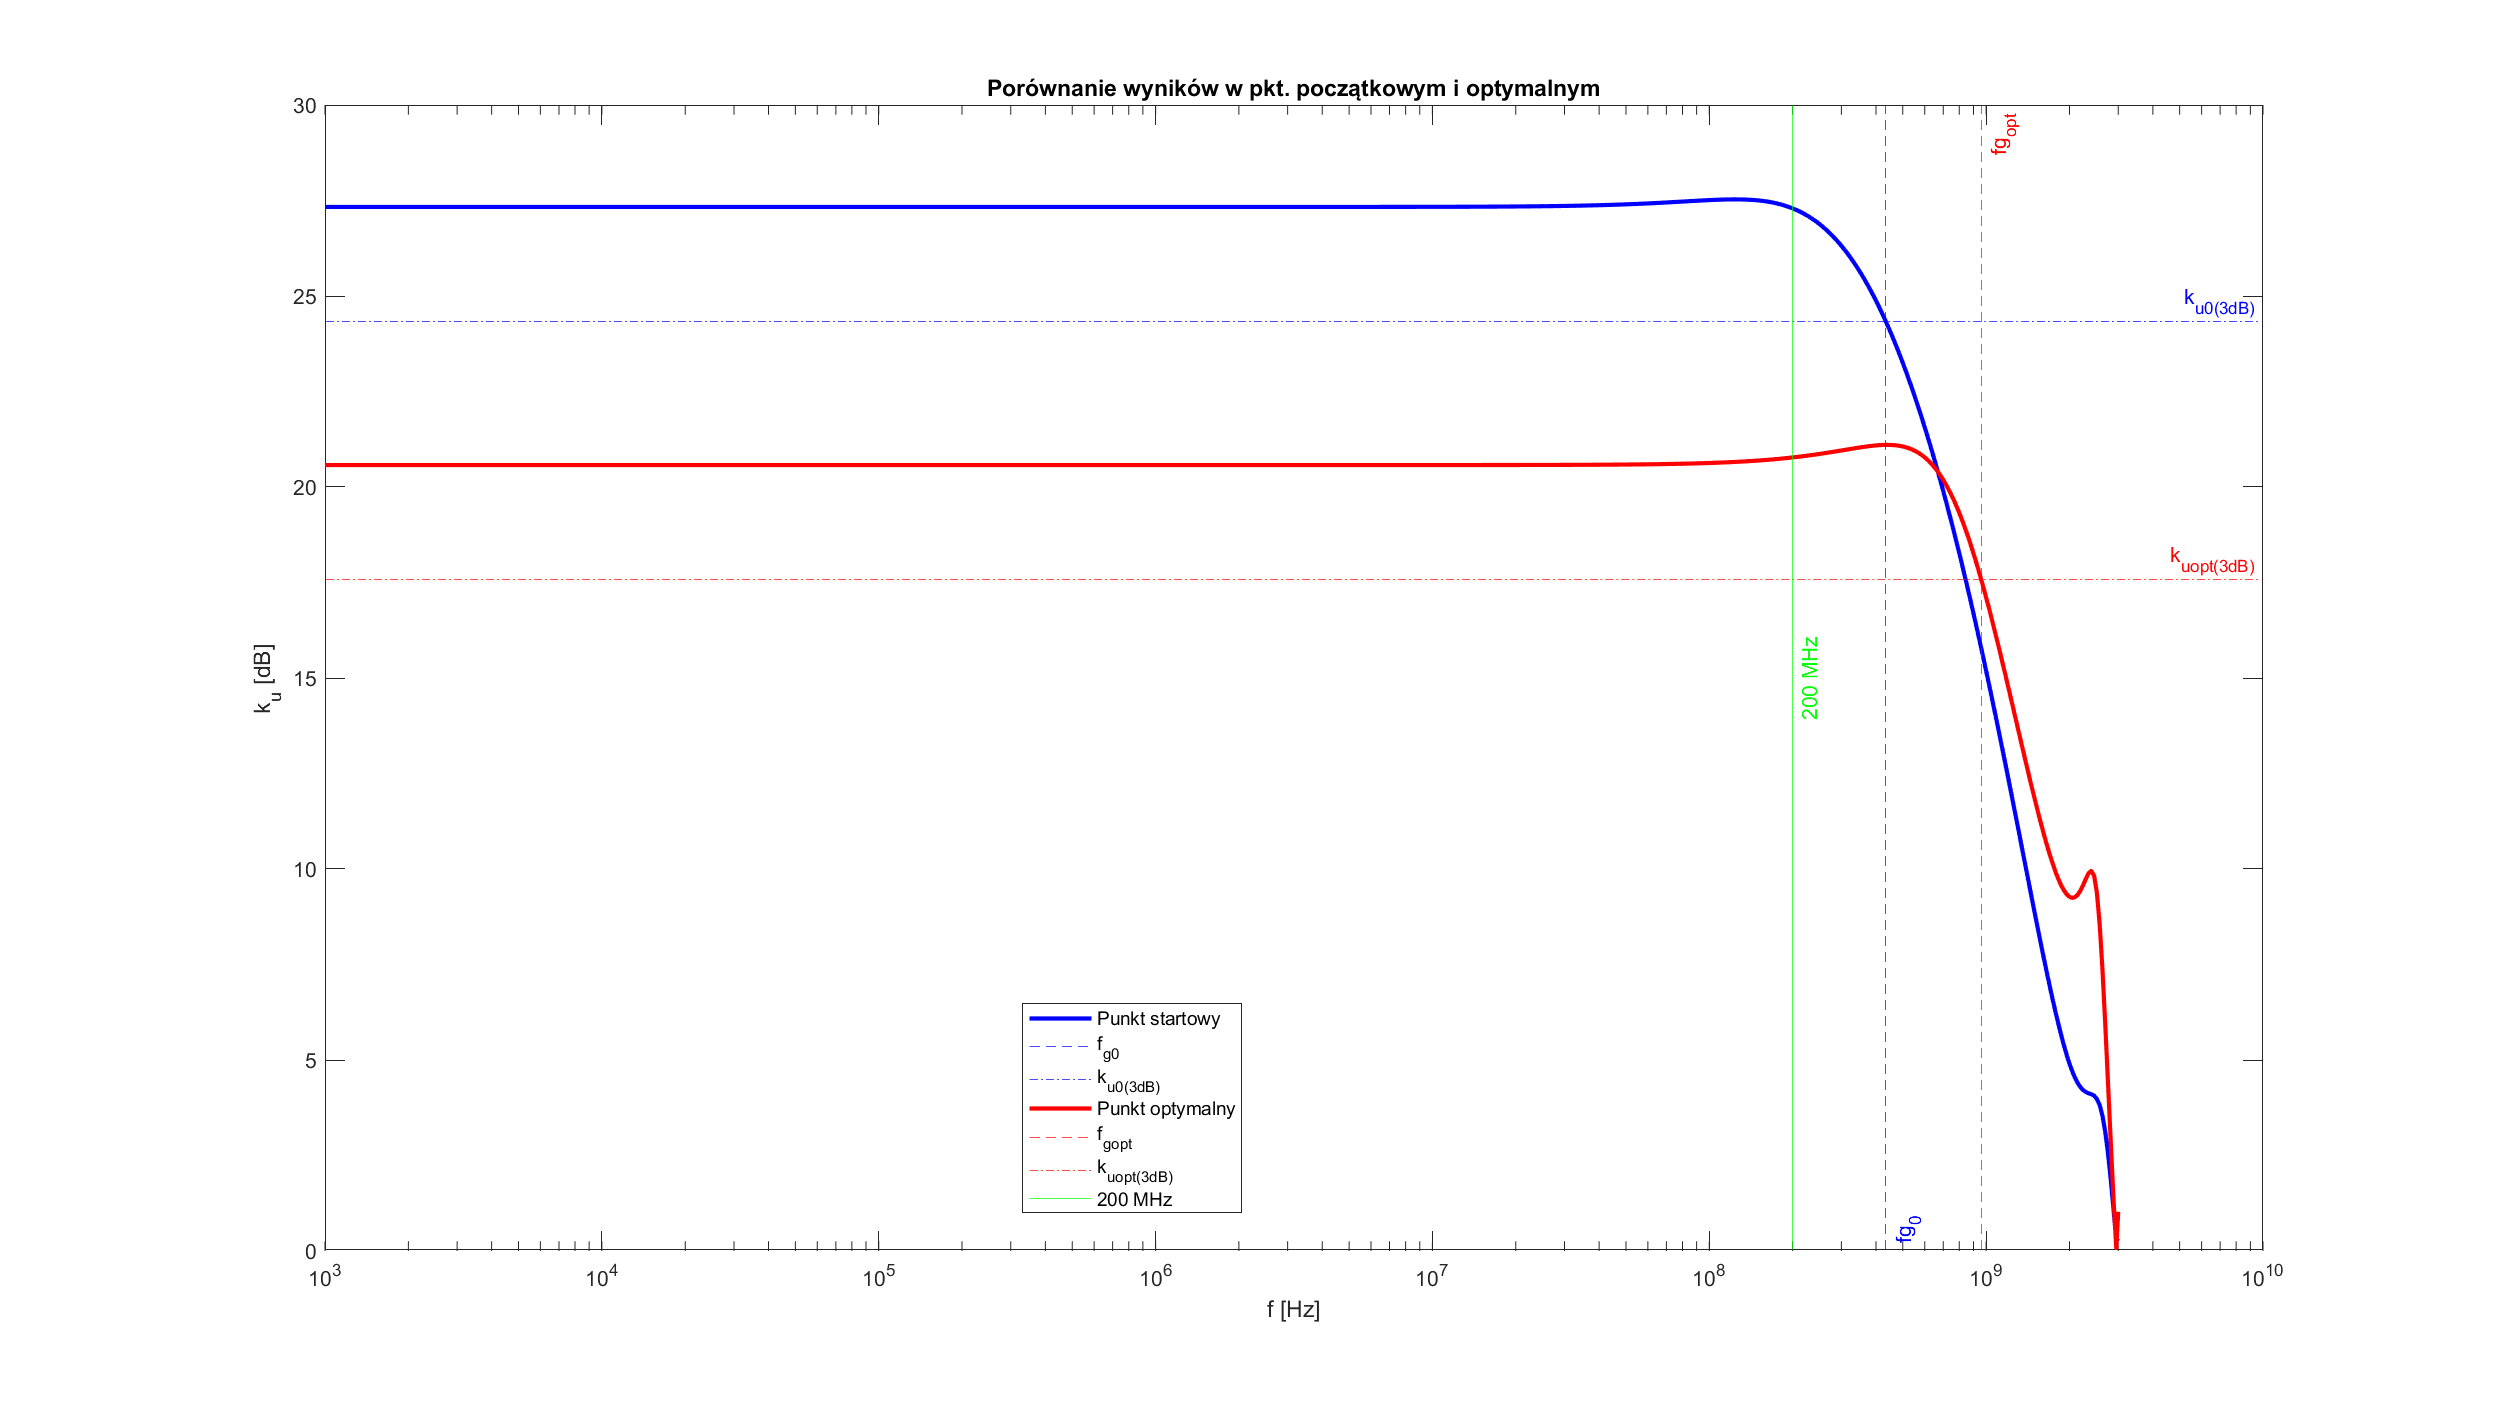
\includegraphics[width=12cm]{graphics/comparison.png}
	\centering
	\caption{Porównanie punktu optymalnego i startowego.}
\end{figure}

\begin{figure}[h]
	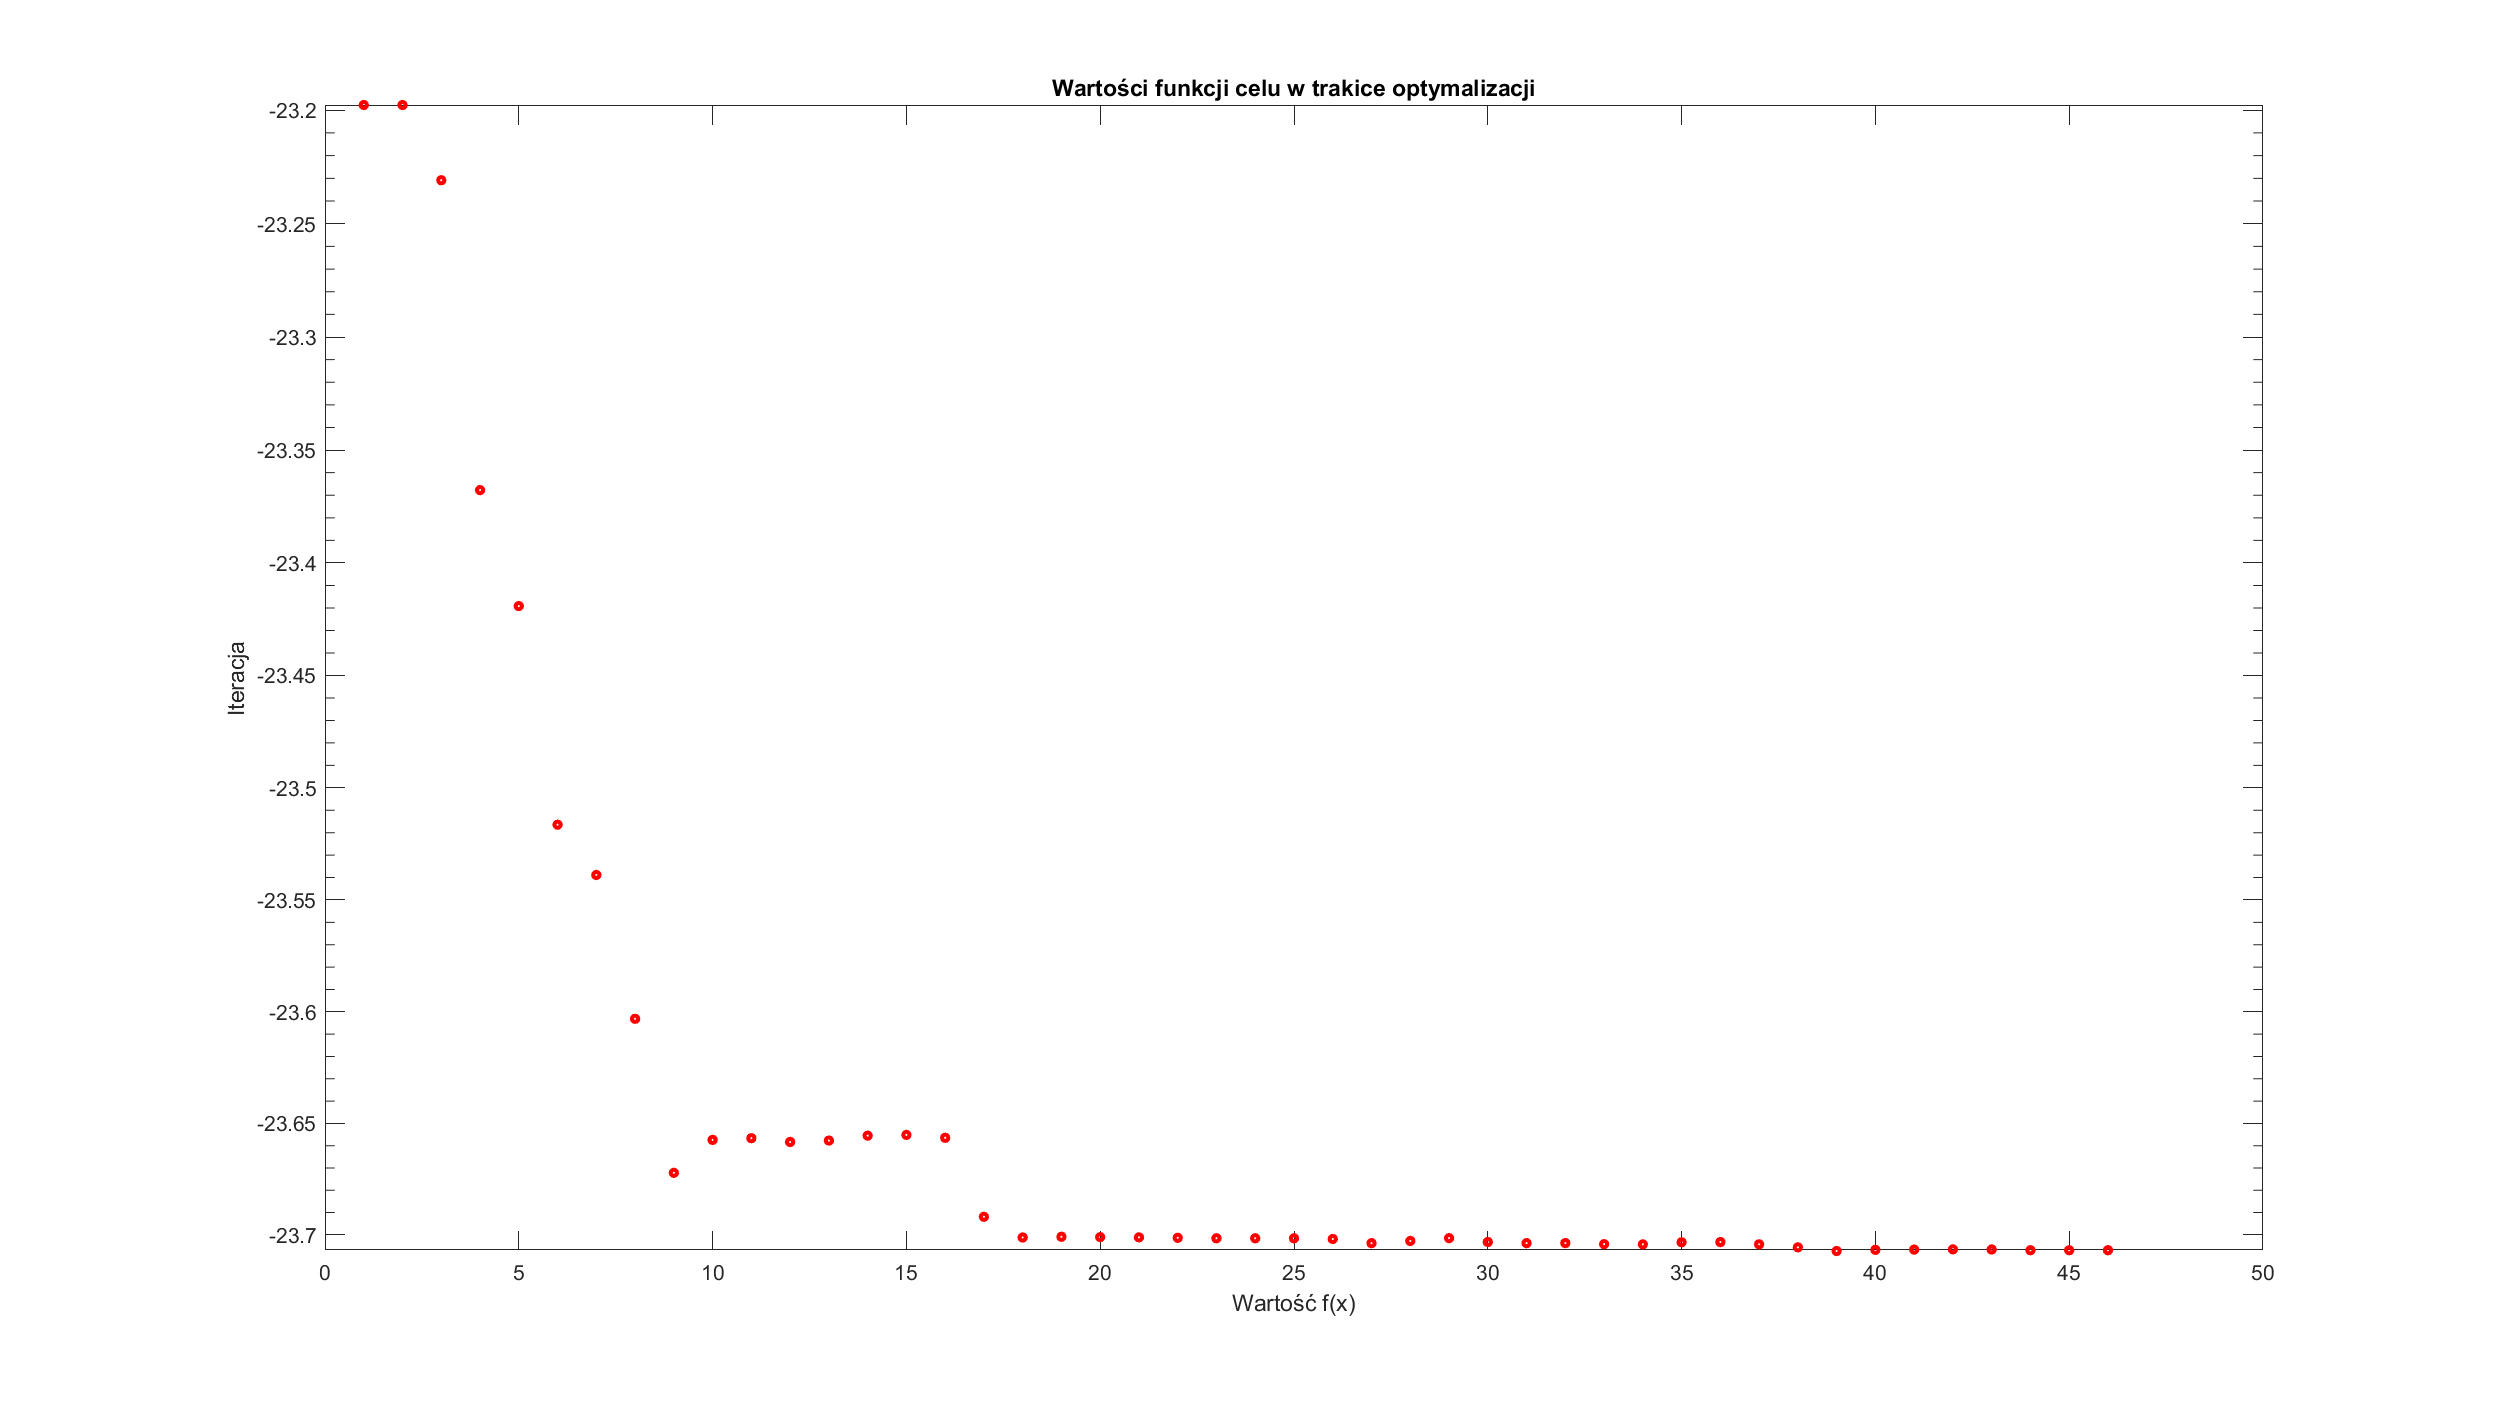
\includegraphics[width=12cm]{graphics/fval.png}
	\centering
	\caption{Przebieg wartości funkcji celu.}
\end{figure}

\begin{figure}[h]
	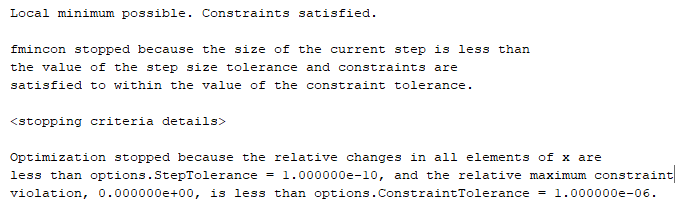
\includegraphics[width=10cm]{graphics/exit_msg.png}
	\centering
	\caption{Informacja o zakończeniu pracy przez optymalizator.}
\end{figure}


\begin{figure}[h]
	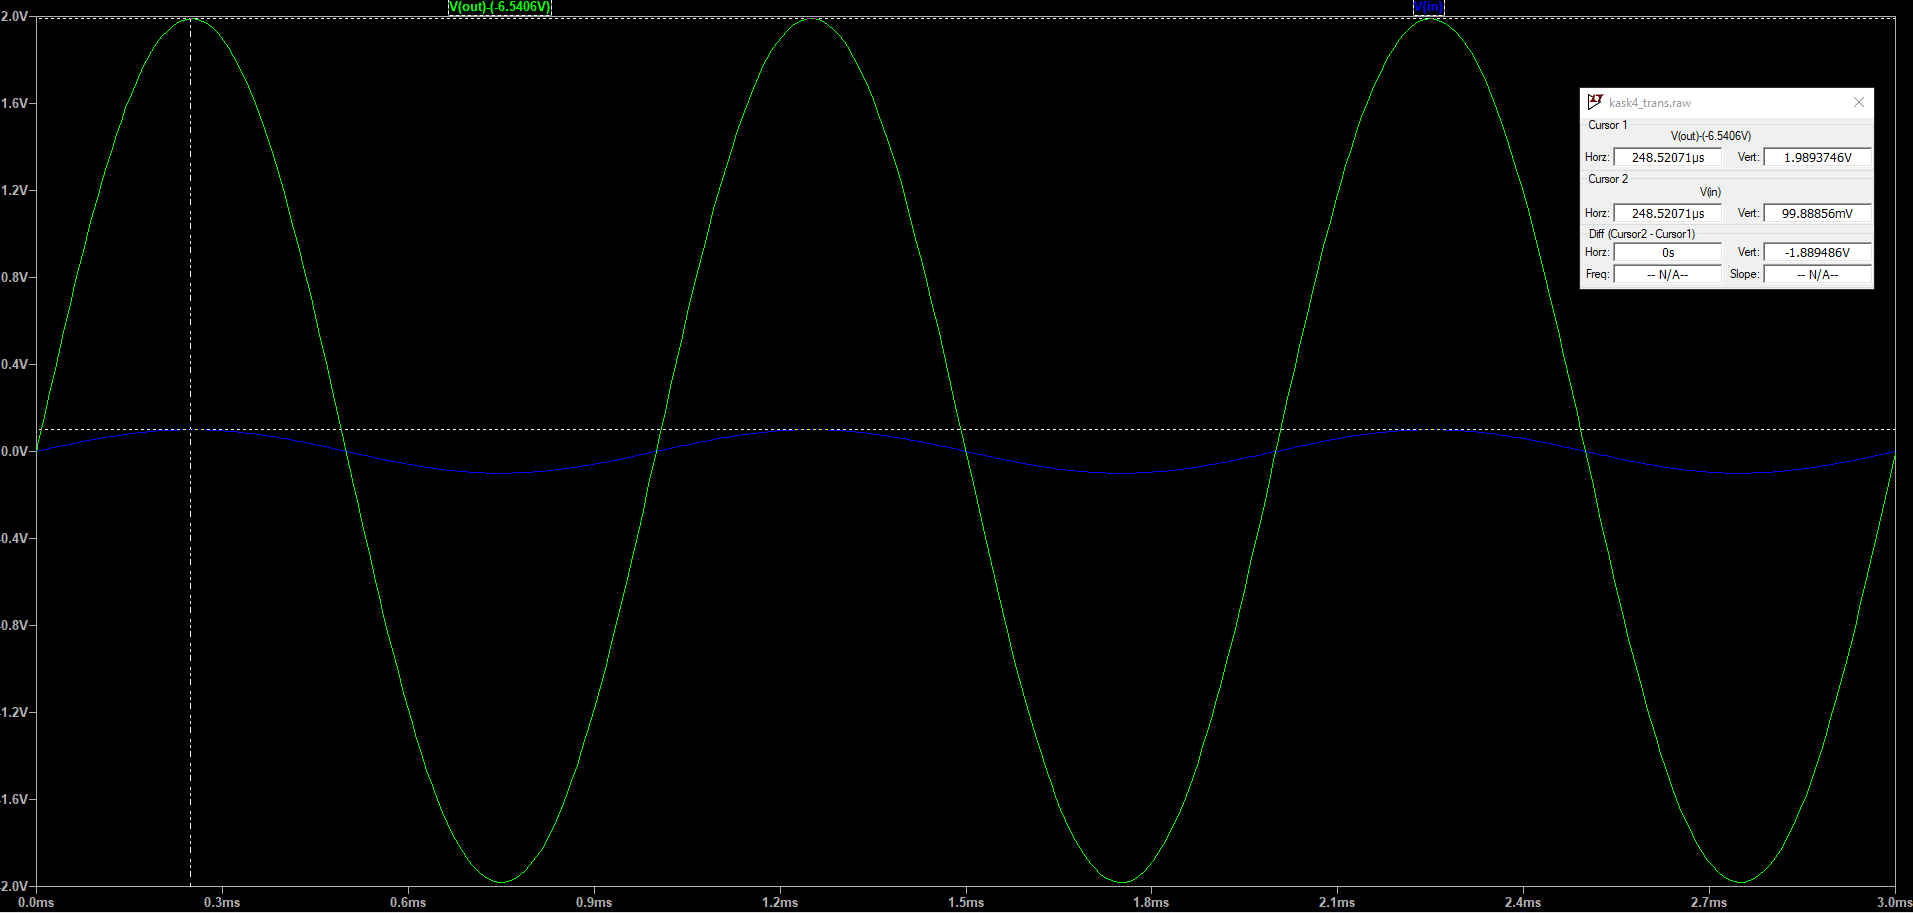
\includegraphics[width=10cm,height=4cm]{graphics/optim_tran.png}
	\centering
	\caption{Symulacja czasowa w pkt. optymalnym. Wzmacniacz wzmacnia.}
\end{figure}


\pagebreak










\clearpage
\begin{center}
	\title{ \huge \textbf{Wykresy w dużej rozdzielczości}}
\end{center}

\begin{landscape}
	\begin{figure}[h]
		\vspace*{-2cm}
		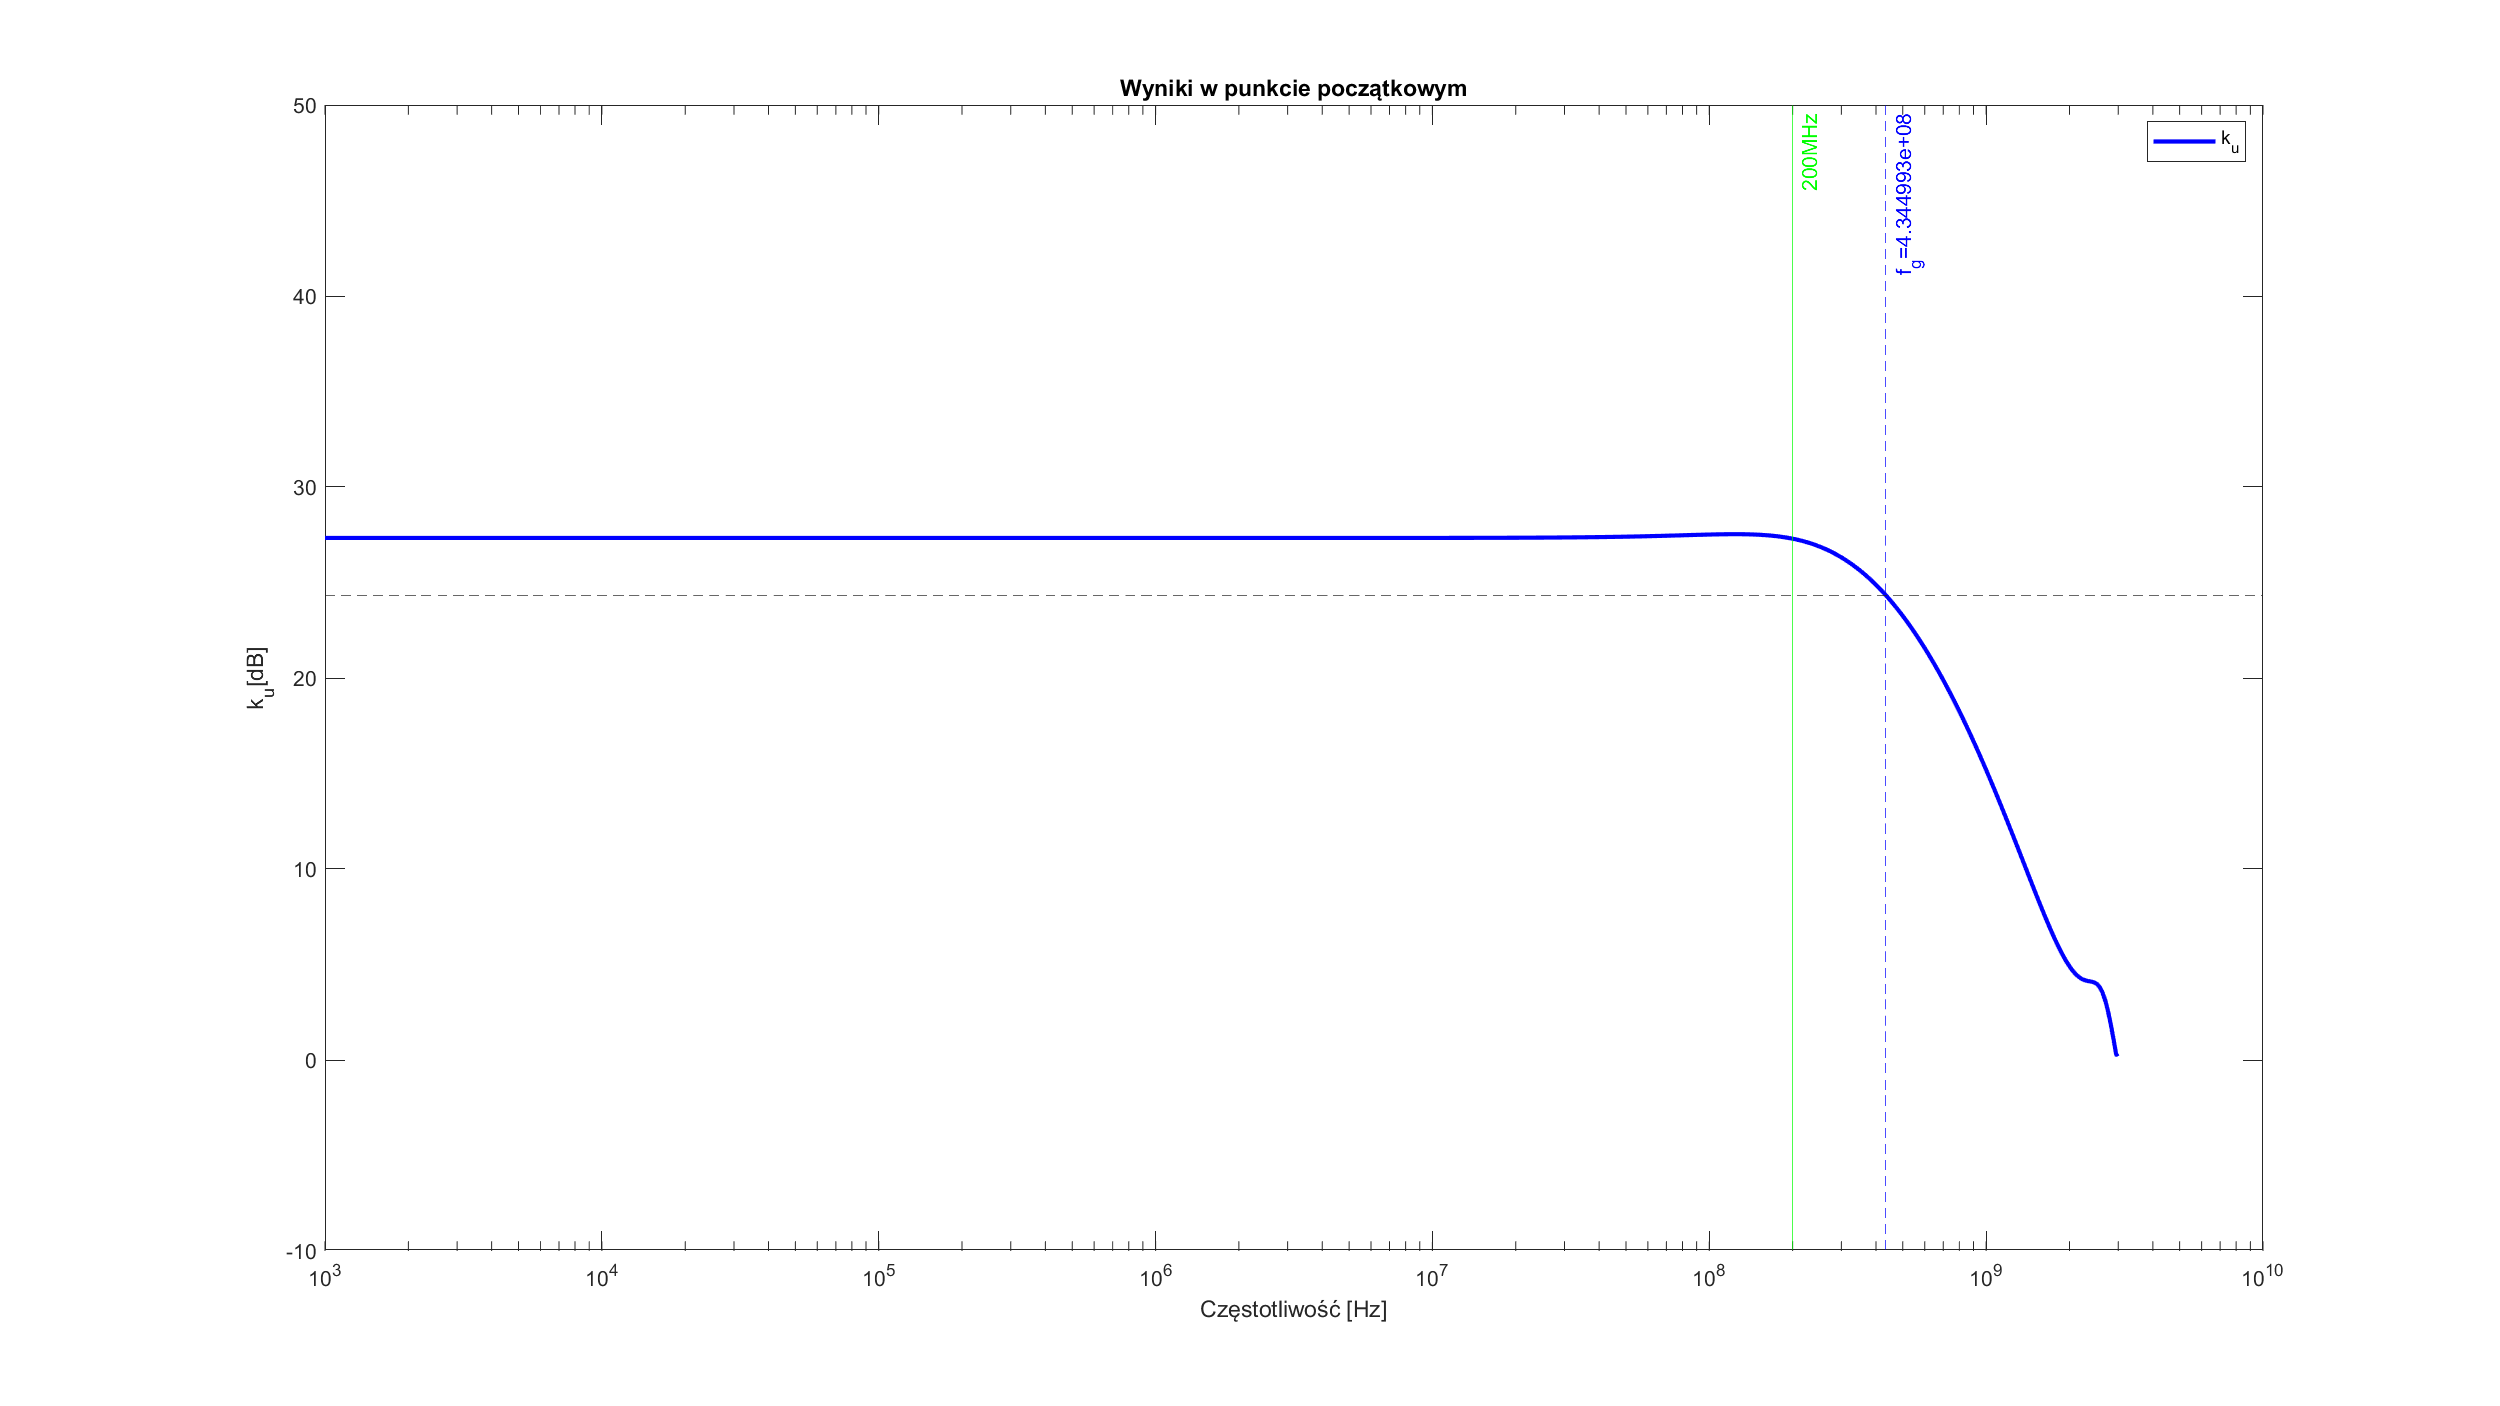
\includegraphics[width=25cm,height=15 cm]{graphics/starting_point.png}
		\centering
		\caption{Charakterystyka układu w punkcie startowym.}
	\end{figure}
\end{landscape}

\clearpage
\pagebreak
\begin{landscape}
	\begin{figure}[h]
		\vspace*{-2cm}
		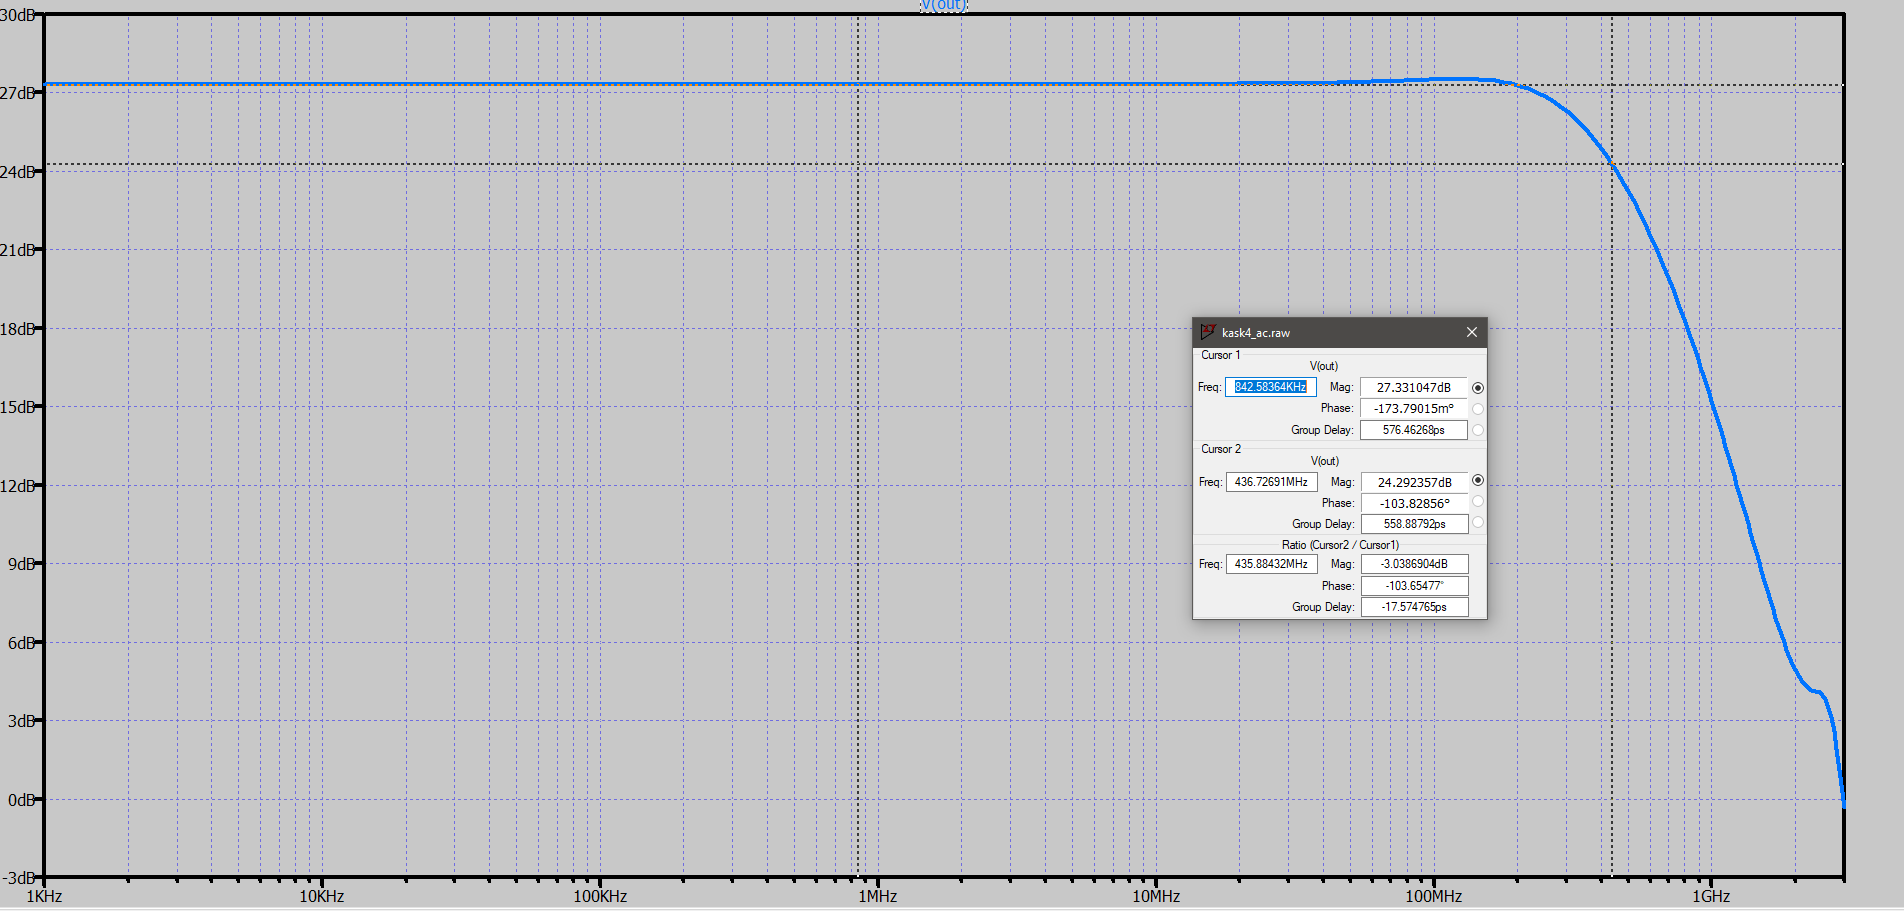
\includegraphics[width=20cm,height=10 cm]{graphics/starting_point_spice.png}
		\centering
		\caption{Charakterystyka układu w punkcie startowym (LTSpice).}
	\end{figure}
\end{landscape}

\pagebreak
\begin{landscape}
	\begin{figure}[h]
		\vspace*{-2cm}
		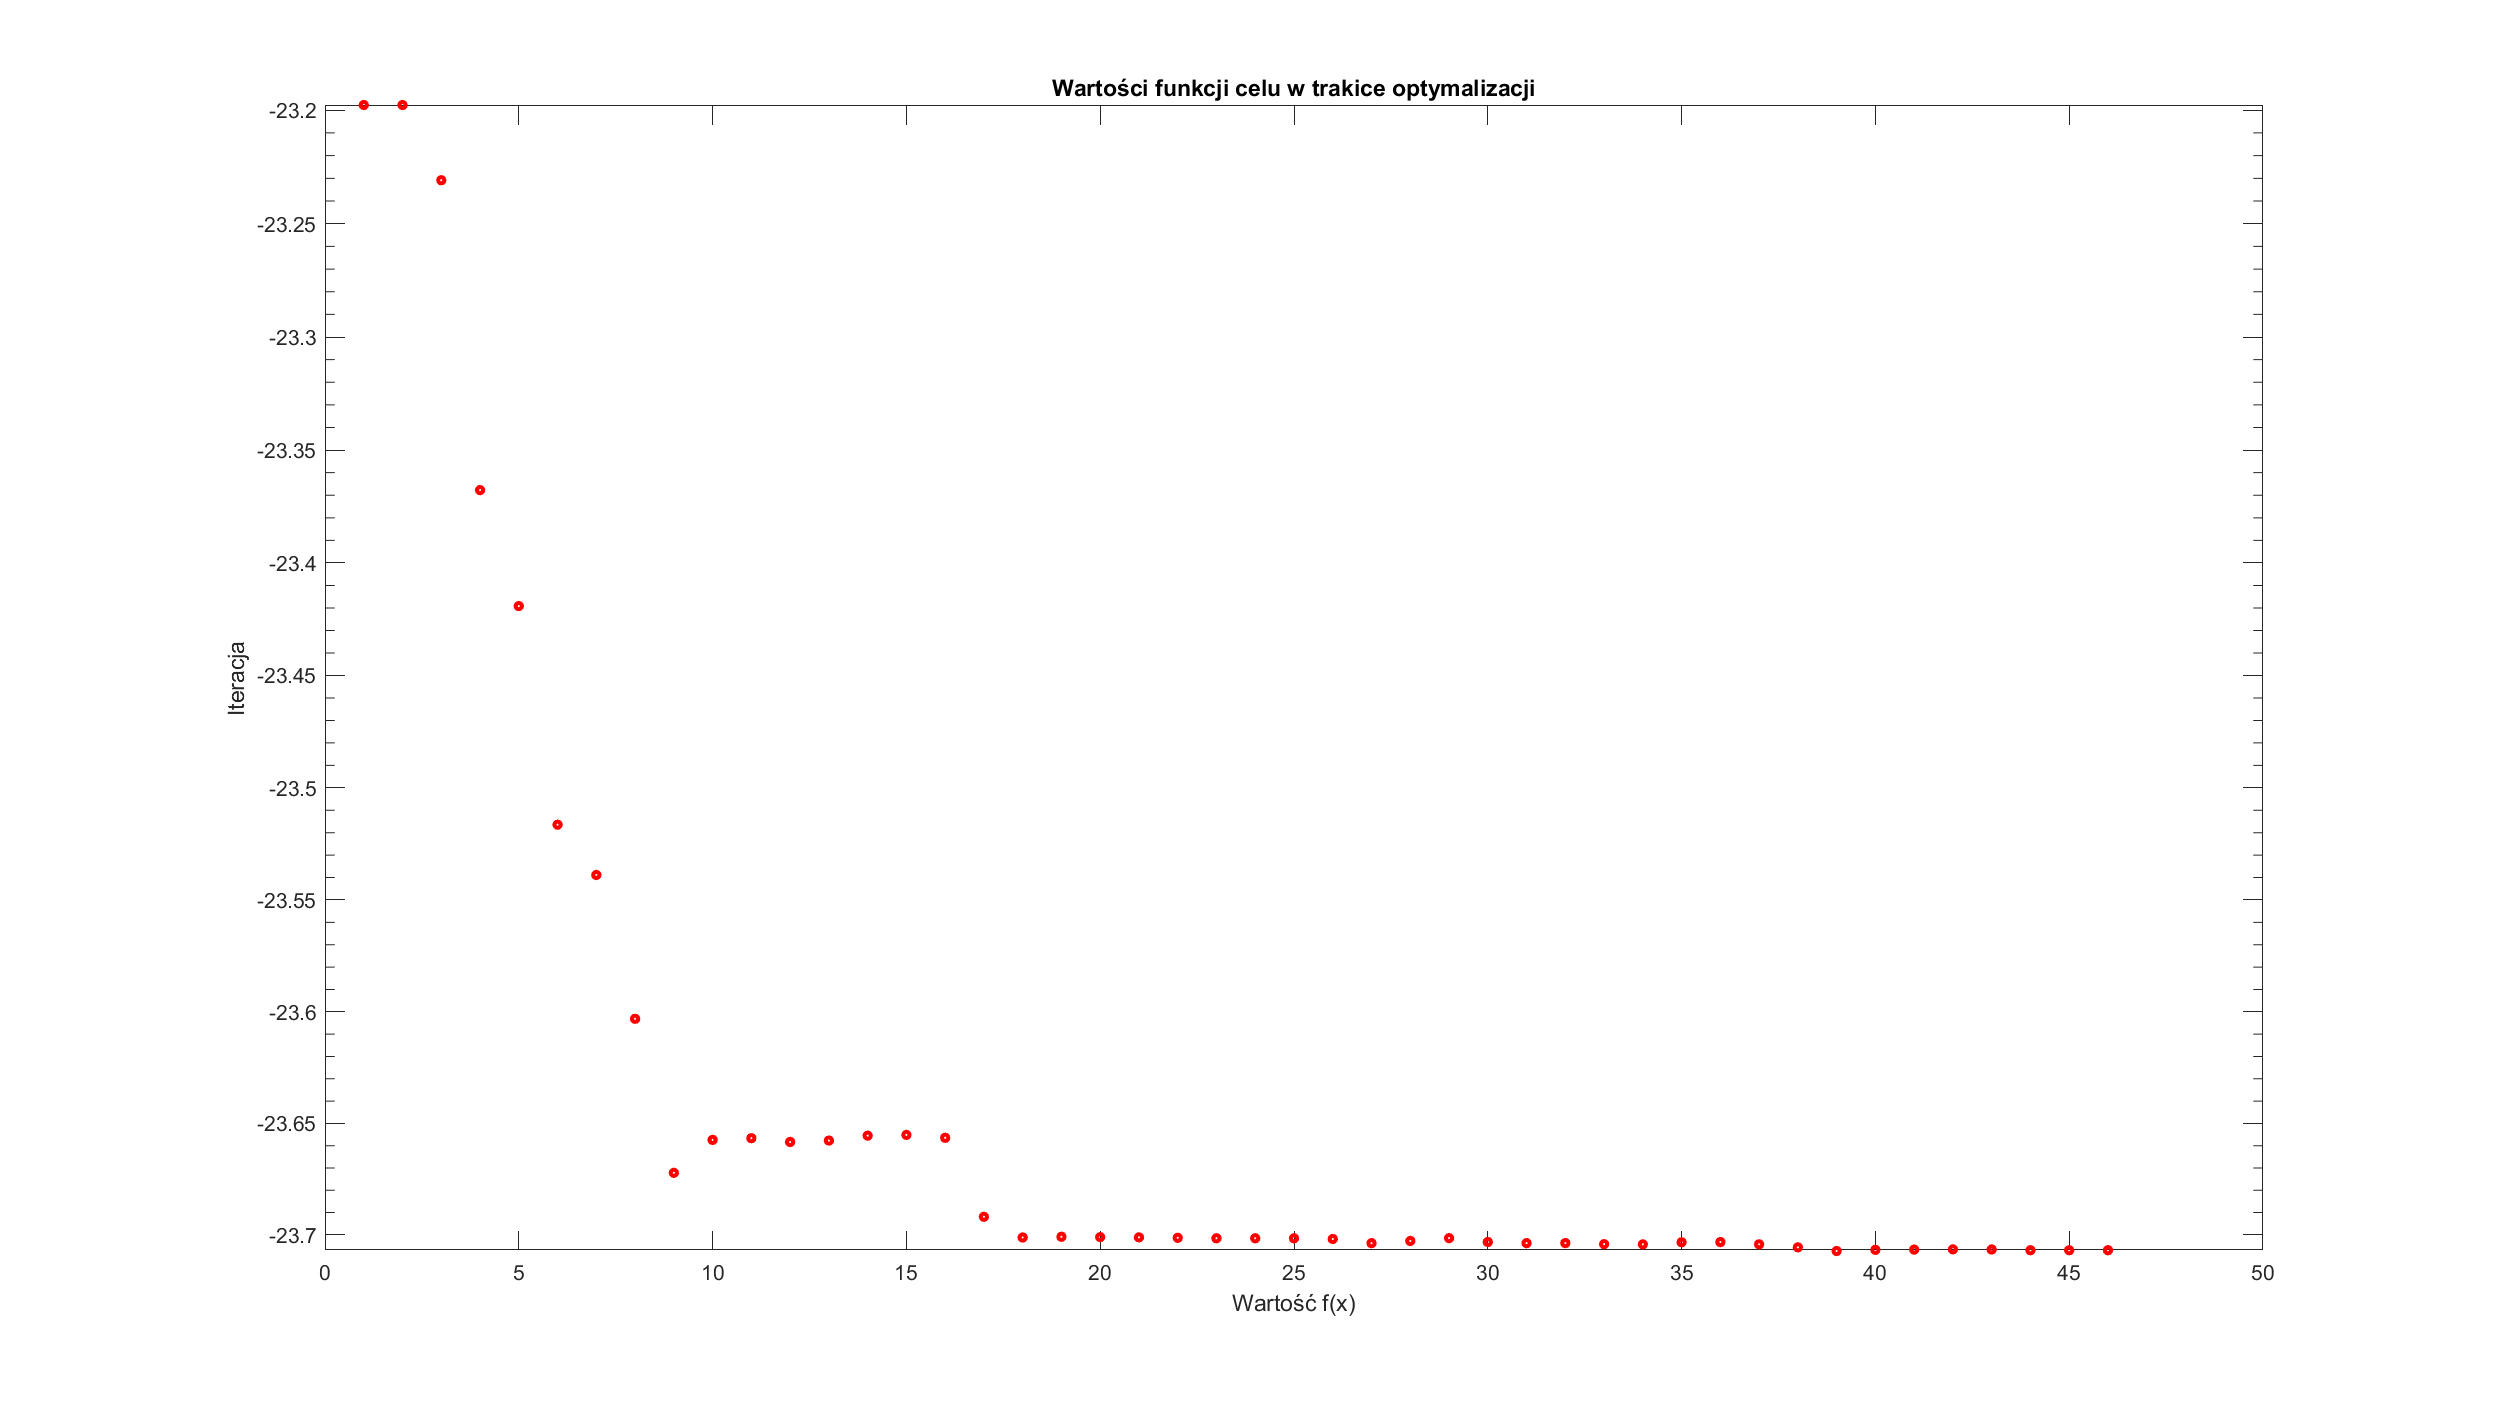
\includegraphics[width=25cm,height=15 cm]{graphics/fval.png}
		\centering
		\caption{Przebieg wartości funkcji celu.}
	\end{figure}
\end{landscape}

\pagebreak
\begin{landscape}
	\begin{figure}[h]
		\vspace*{-2cm}
		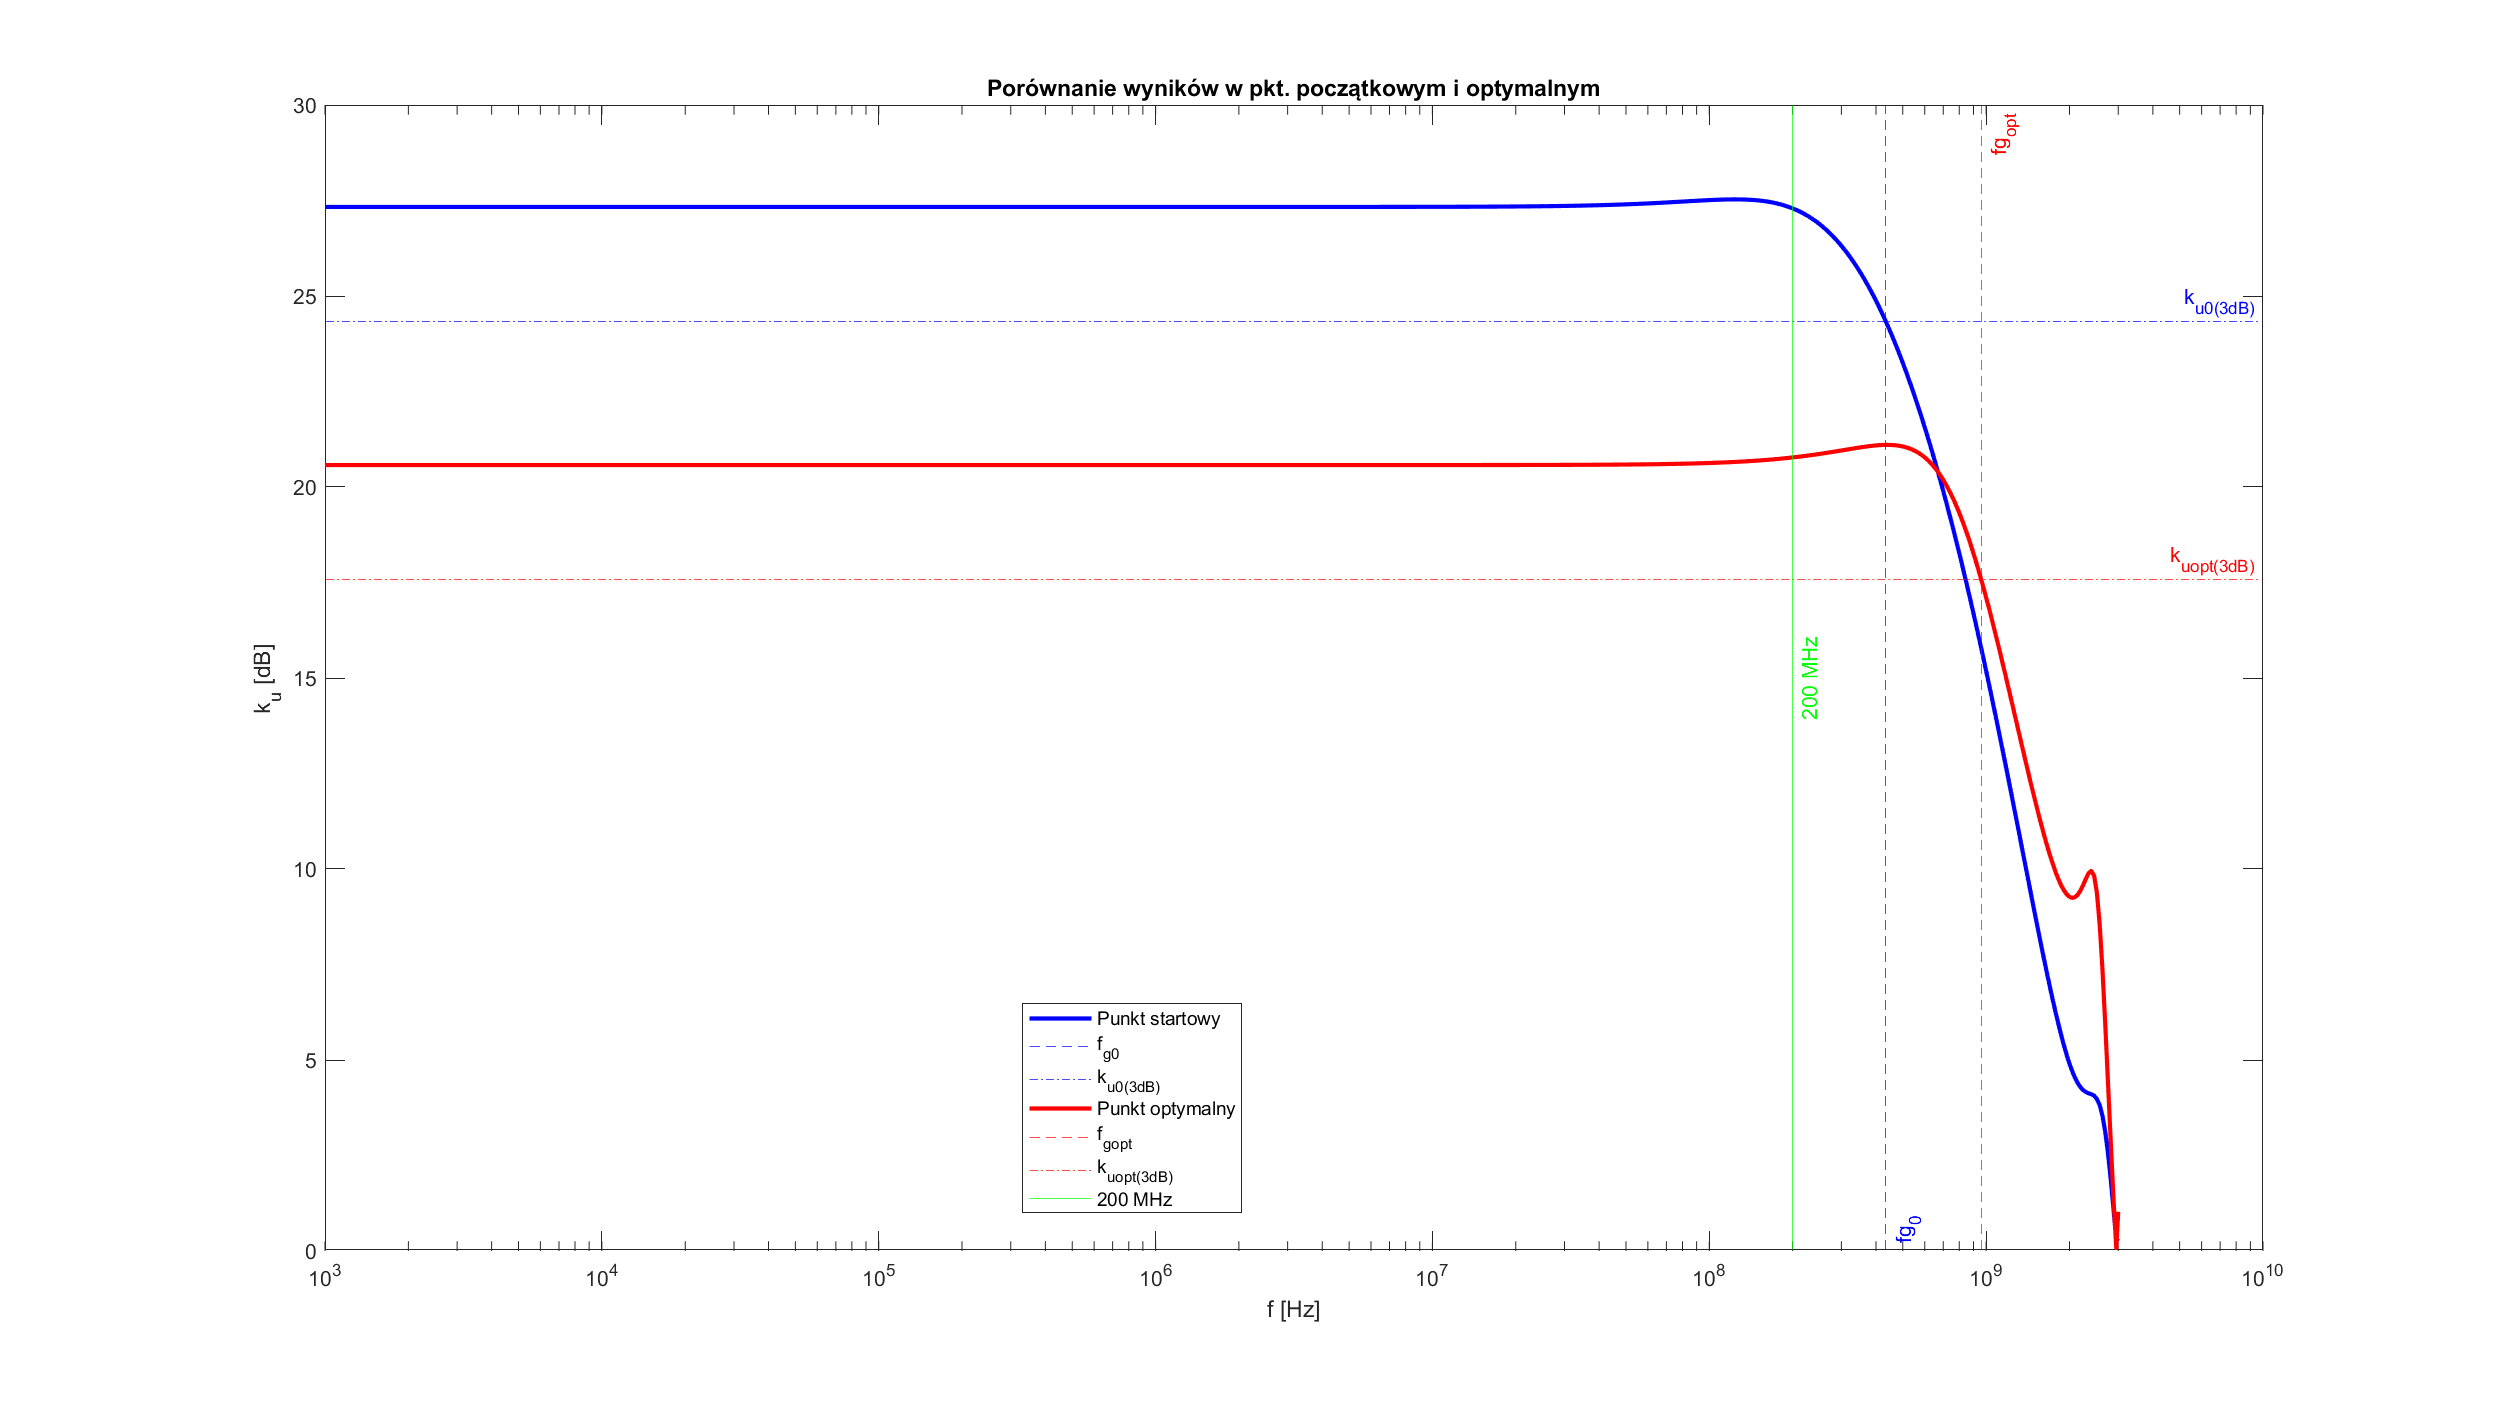
\includegraphics[width=25cm,height=15 cm]{graphics/comparison.png}
		\centering
		\caption{Porównanie wyników w punkcie optymalnym i startowym.}
	\end{figure}
\end{landscape}

\pagebreak
\begin{landscape}
	\begin{figure}[h]
		\vspace*{-2cm}
		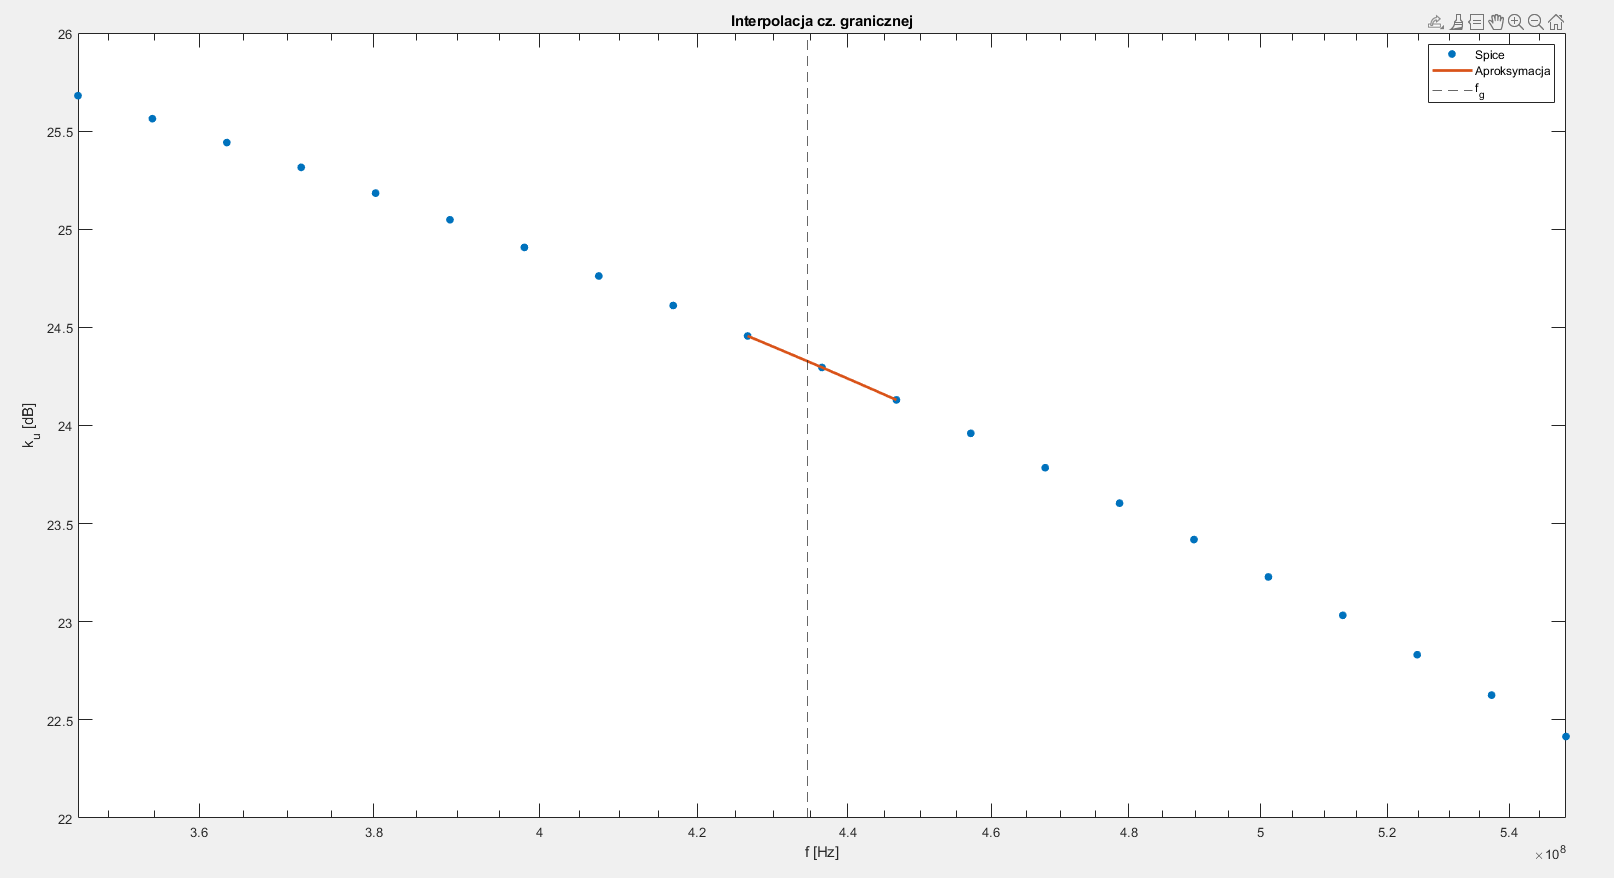
\includegraphics[width=20cm,height=10 cm]{graphics/fg_interp.png}
		\centering
		\caption{Interpolacja częstotliwości granicznej.}
	\end{figure}
\end{landscape}

\pagebreak
\begin{landscape}
	\begin{figure}[h]
		\vspace*{-2cm}
		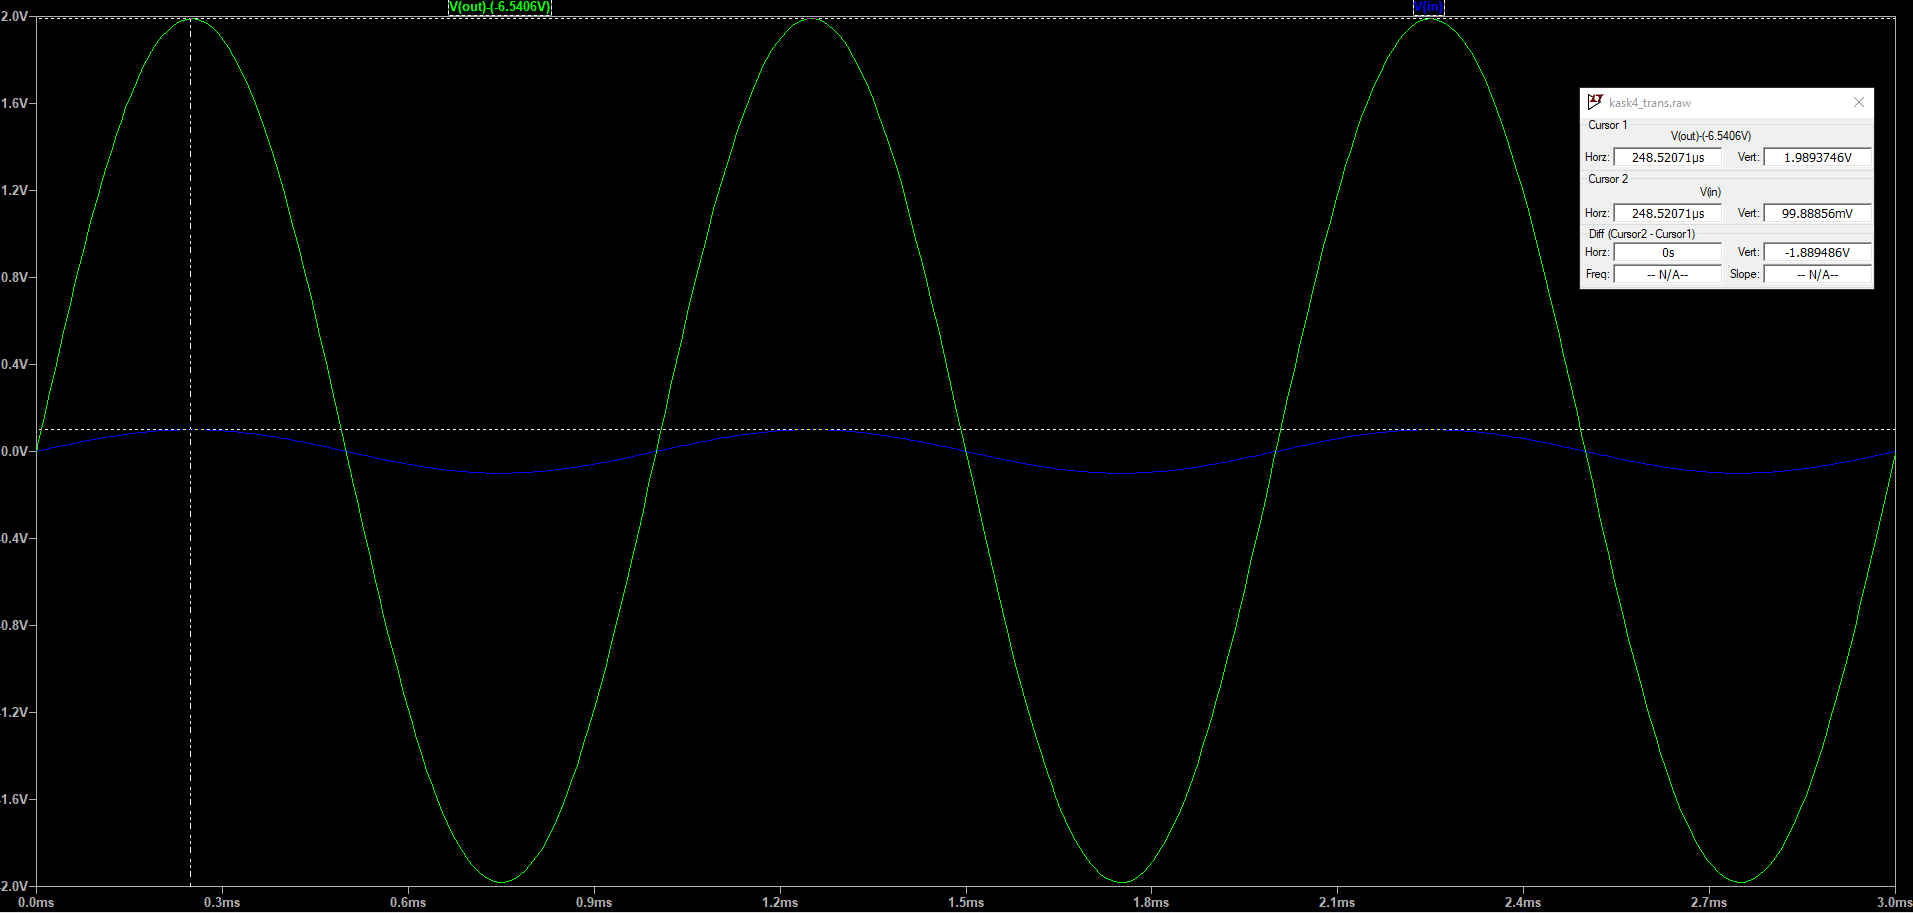
\includegraphics[width=20cm,height=10cm]{graphics/optim_tran.png}
	\centering
	\caption{Symulacja czasowa w pkt. optymalnym. Wzmacniacz wzmacnia.}
	\end{figure}
\end{landscape}

\end{document}


